%%%%%%%%%%%%%%%%%%%%%%%%%%%%%%%%%%%%%%%%%%%%%%%%%%%%%%%%%%%%%%%%%%%%%%%%%%%%%%%%
%neutrino_physics.tex: Chapter on neutrino physics:
%%%%%%%%%%%%%%%%%%%%%%%%%%%%%%%%%%%%%%%%%%%%%%%%%%%%%%%%%%%%%%%%%%%%%%%%%%%%%%%%
\chapter{Theoretical Motivations}
\label{wrBosonAndHeavyNu}
%%%%%%%%%%%%%%%%%%%%%%%%%%%%%%%%%%%%%%%%%%%%%%%%%%%%%%%%%%%%%%%%%%%%%%%%%%%%%%%%
Experimental evidence \cite{NOvAresults,mainzPhaseIIResults,t2kResults} of neutrinos with non-zero masses motivated extensions to the Standard Model (SM).  
Before discussing SM extensions, the methods through which the weak bosons $W^{\pm},Z$ and fermions acquired mass 
in the SM are discussed.  Subsequently, a SM extension is presented to explain neutrino masses using the 
mass generation methods of the SM, and other experimentally observed phenomena not explained by the SM.  
The chapter concludes by presenting phenomenological aspects of the SM extension relevant to experimental 
detection.

\section{Particle Masses in the Standard Model}
\label{sec:massInSM}
The SM postulated that the four generators of the $SU(2)_{L} \times U(1)$ groups transformed into the massless 
photon and massive $W^{\pm}$ and $Z$ bosons through the Brout-Englert-Higgs (BEH) mechanism.  This mechanism 
added four degrees of freedom to the SM, in the form of a complex doublet $\Phi$ representing four bosonic 
particles, which obey the Lagrangian $\Ell_{H}$:

\begin{align}
	\Phi &= \begin{bmatrix}
	\phi^{+} \\
	\phi^{0}
	\end{bmatrix}
\end{align}

\begin{equation}
	\Ell_{H} = (D_{\mu}\Phi)^{\dagger}D^{\mu}\Phi - V(\Phi)
\end{equation}

where $V(\Phi) = \frac{1}{2}(|\Phi|^{2} - \frac{\nu^{2}}{2})$ was the Higgs potential, and 
$D_{\mu} = \partial_{\mu} + ig_{L}\tau^{j}A^{j}_{\mu} + i\frac{g'}{2}YB_{\mu}$ described the propagation 
of the Higgs doublet $\Phi$ and its couplings to the $SU(2)_L$ generators $\tau^{j}$ and massless vector 
fields $A^{j}_{\mu}$, and the $U(1)$ generator $Y$ and massless vector field $B_{\mu}$.  $g_{L}$ and 
$g'$ set the weak and electromagnetic interaction coupling strengths.  The Higgs doublet $\Phi$ took a 
value $<\Phi> =$ (0  $\nu/\sqrt{2}$) to minimize the Higgs potential, after which the $\Ell_{H}$ reduced 
to:

\begin{equation}
	\Ell_{HK} = \frac{\nu^{2}}{8}[g^{2}_{L}(A^{1}_{\mu} + iA^{2}_{\mu})(A^{1\mu} - iA^{2\mu}) + (g'B_{\mu} - g_{L}A^{3}_{\mu})^{2}]
\end{equation}

The photon vector field $A_{\mu}$, and the weak boson vector fields $W^{\pm}_{\mu}$ and $Z_{\mu}$ were defined as:

\begin{equation}
	W^{\pm}_{\mu} \equiv \frac{1}{\sqrt{2}}(A^{1}_{\mu} \pm iA^{2}_{\mu}), 
	Z_{\mu} \equiv \frac{1}{\sqrt{g'^{2} + g^{2}_{L}}}(g'B_{\mu} - g_{L}A^{3}_{\mu}), 
	A_{\mu} \equiv \frac{1}{\sqrt{g'^{2} + g^{2}_{L}}}(g_{L}B_{\mu} + g'A^{3}_{\mu})
\end{equation}

transformed $\Ell_{H}$ into:

\begin{equation}
	\Ell_{HK} = (\frac{\nu g_{L}}{2})^{2}W^{+}_{\mu}W^{-\mu} + \frac{1}{2}(\frac{\nu \bar{g}}{2})^{2}Z_{\mu}Z^{\mu} + 0A_{\mu}A^{\mu}
\end{equation}

where $\bar{g} \equiv \sqrt{g'^{2} + g^{2}_{L}}$.  Following from this Lagrangian, the photon $A_{\mu}$ was massless, 
the $Z$ boson had mass $m_{Z} = \nu\bar{g}/2$, and the $W^{\pm}$ bosons had mass $m_{W} = \nu g_{L}/2$.  
Three of the four scalar fields introduced by the BEH mechanism were consumed and gave mass to the $Z$ 
and $W^{\pm}$ bosons.  Recent experimental evidence of the fourth scalar field \cite{combinedHiggsResult}, the Higgs boson, 
supported the SM prediction that the $Z$ and $W^{\pm}$ bosons acquired mass through the BEH mechanism.

Experimental evidence supported the prediction that quarks and charged leptons are massive particles.  In the SM, they could acquire mass 
through two methods.  Their masses could be added directly to the SM Lagrangian, or additional Higgs fields 
could be added to the BEH mechanism.  In either case, the result was mass terms of the form $-mf\bar{f}$, where $f$ is a fermion 
representing a quark or charged lepton, were added to the SM Lagrangian.  In the basis where a 
fermion field $f$ consisted of a right-handed component $\chi_{R}$ and left-handed 
component $\chi_{L}$, $f = (\chi_{L},\chi_{R})$, a fermion mass term in the SM Lagrangian was written as:

\begin{equation}
	\Ell_{D} = -m\bar{f}f = -m\chi^{\dagger}_{L}\chi_{R} - m\chi^{\dagger}_{R}\chi_{L}
\end{equation}

This type of mass term, called a Dirac mass, contained the product of left and right-handed fields.  Experimental 
evidence substantiated that quarks and charged leptons, or their anti-particles, were massive and could be left or right-handed 
fields.  Their masses were assigned using Dirac mass terms.

Neutrinos played a special role in the SM.  The SM postulated that they are neutral, massless fermions, and only interacted 
with other particles through the weak interaction.  In addition, due to parity violation of the weak interaction, 
anti-neutrinos $\bar{\nu_{\ell}}$ were always right-handed, and neutrinos $\nu_{\ell}$ were always left-handed.  Fermions in 
the SM acquired mass through a Lagrangian of the form $\Ell_{D}$, which could not be used to explain SM neutrino masses 
due to the multiplication of left and right-handed fields.  An extension of the SM was needed to explain neutrino masses.


\section{Standard Model Extensions}
\label{sec:lrsExtensions}
Several SM extensions accommodated massive neutrinos.  One of the simplest extensions proposed that neutrinos 
were Majorana fermions, instead of Dirac fermions as in the SM.  Majorana neutrinos, first proposed 
in 1937 \cite{majoranaTheory}, were fermions that were their own anti-particles, and had masses 
$m_{L},m_{R}$ given by the Lagrangian $\Ell_{M}$:

\begin{equation}
	\Ell_{M} = -m_{L}\chi^{\dagger}_{L}\chi_{L} - m_{R}\chi^{\dagger}_{R}\chi_{R}
\end{equation}

The Majorana masses could be generated through an extended Higgs model, or adding terms of the form $\Ell_{M}$ 
to the SM Lagrangian.  If light Majorana neutrinos existed, then the double beta decay process could occur 
with no neutrinos.  Experimental evidence of neutrinoless double beta decay was not found 
\cite{igexDblBetaDecay,gerdaDblBetaDecay}, so a different SM extension was needed to explain neutrino masses.

Another class of SM extensions that explained the origin of neutrino masses were Left-Right Symmetric (LRS) extensions.  
First proposed in 1974 \cite{earlyLRSModel}, LRS models postulated that a precursor to the SM electromagnetic and weak interactions 
existed in the very early universe, conserved parity and was mediated by seven massless gauge bosons.  
Shortly after the Big Bang an extension of the SM BEH mechanism transformed the seven massless gauge bosons 
into the massless photon, the SM $W^{\pm}$ and $Z$ bosons, and three heavier bosons $W^{\pm}_{R}$ (\WR) and $Z'$.  
The mechanism through which the SM $W^{\pm}$ and $Z$, and \WR and $Z'$ bosons acquired mass is discussed next, and 
is followed by a discussion of neutrino masses in LRS models.

The subset of LRS models considered here added a $SU(2)_{R}$ group to the SM $SU(2)_{L} \times U(1)$ groups.
Adding the $SU(2)_{R}$ group to the SM introduced three new, massless vector fields $\xi^{j}_{\mu}$.  In these LRS models, 
the SM BEH mechanism is extended in two stages, and created six massive gauge bosons that mediated the weak interaction.  
In the first stage \cite{lrsHiggsStageOne}, a chiral, complex Higgs doublet $\chi_{L,R}$ was introduced 

\begin{align}
	\chi_{L,R} &= \begin{bmatrix}
	\chi^{+}_{L,R} \\
	\chi^{0}_{L,R}
	\end{bmatrix}
	\label{eq:stageOneVEV}
\end{align}

with bosonic fields that coupled independently to left and right-handed gauge bosons.  The propagation and interaction of these 
fields with other massless bosons was described by the Lagrangian:

\begin{equation}
	\Ell_{H,LRS} = \frac{1}{2}(D_{\mu}\chi_{L})^{\dagger}D^{\mu}\chi_{L} + \frac{1}{2}(D_{\mu}\chi_{R})^{\dagger}D^{\mu}\chi_{R} - V(\chi_{L,R})
\end{equation}

where $D_{\mu} = \partial_{\mu} + ig_{L}\tau^{j}A^{j}_{L\mu} + ig_{R}\tau^{j}\xi^{j}_{R\mu} + i\frac{g'}{2}YB_{\mu}$ contains 
the massless boson fields $A^{j}_{L\mu}, \xi^{j}_{R\mu}, B_{\mu}$ multiplied by the generators of the $SU(2)_{L}, SU(2)_{R}, U(1)$ groups.  
In the LRS models considered here the coupling strengths $g_{R}, g_{L}$ were assumed to be equal, and denoted as $g$.  
The potential $V(\chi_{L,R})$ respects the symmetries of LRS models, depends on a constant $U_{R}$, and was minimized when $\chi_{L,R}$ 
took values $<\chi^{+}_{L,R}> = 0, <\chi^{0}_{L}> = 0, <\chi^{0}_{R}> = U_{R}$.  In the early universe $V(\chi_{L,R})$ was minimized, and 
subsequently new, massive fields were created.  The new fields:

\begin{equation}
	W^{\pm}_{R\mu} \equiv \frac{1}{\sqrt{2}}(\xi^{1}_{R\mu} \mp i\xi^{2}_{R\mu}), 
	Z'_{\mu} \equiv \frac{1}{\sqrt{g'^{2} + g^{2}}}(-g'B_{\mu} + g\xi^{3}_{R\mu})
\end{equation}

acquired masses:

\begin{equation}
	\Ell_{HK,LRS} = (\frac{1}{4}U^{2}_{R}g^{2})W^{+\mu}_{R}W^{-}_{R\mu} + \frac{1}{2}[\frac{1}{4}U^{2}_{R}(g^{2} + g'^{2})]Z'_{\mu}Z'^{\mu}
\end{equation}

Thus in the first stage extension of the BEH mechanism, the bosons $W^{\pm}_{R}, Z'$ were created with masses $m_{W_{R}} = \frac{1}{2}gU_{R}$ 
and $m_{Z'} = \frac{1}{2}U_{R}\sqrt{g'^{2} + g^{2}}$, and all other bosons remained massless.

Following the first stage, the second stage extension of the BEH mechanism \cite{lrsHiggsStageOne,lrsHiggsStageTwo} introduced two complex Higgs doublets 
$\phi_{1}$ and $\phi_{2}$ represented by the multiplet $\Phi$:

\begin{align}
	\Phi &= \begin{bmatrix}
	\phi^{0}_{1} & \phi^{+}_{2} \\
	\phi^{-}_{1} & \phi^{0}_{2}
	\end{bmatrix}
\end{align}

The multiplet interacted with the left and right-handed $SU(2)$ boson fields, and the Lagrangian $\Ell_{H2,LRS}$ that 
describes\footnote{$\Ell_{H2,LRS}$ is similar to $\Ell_{H}$ described in the previous section, but with extra terms for the second Higgs doublet} these 
interactions included a potential $V(\phi_{1},\phi_{2})$ that forced $\Phi$ to a non-zero expectation value.  When $V(\phi_{1},\phi_{2})$ was 
minimized in the early universe, the multiplet $\Phi$ took the value:

\begin{align}
	<\Phi> &= \begin{bmatrix}
	\nu_{1} & 0 \\
	0 & \nu_{2}
	\end{bmatrix}
	\label{eq:stageTwoVEV}
\end{align}

and the \WR, $Z'$, SM $W^{\pm}$ and $Z$ acquired masses:

\begin{equation}
	m_{W_{L}} = \frac{1}{2}g\nu ,\quad m_{W_{R}} \simeq \frac{1}{2}gU_{R} ,\quad m_{Z} = \frac{1}{2}\bar{g}\nu ,\quad m_{Z'} \simeq \frac{1}{2}\bar{g}U_{R}
\end{equation}
\begin{equation}
	\nu^{2} \equiv \nu^{2}_{1} + \nu^{2}_{2} , \bar{g}^{2} \equiv g^{2} + g'^{2}
\end{equation}

where it was assumed that $U_{R} \gg \nu$, and there was negligible mixing between left and right-handed leptons, 
which is discussed later.  Thus, LRS models predicted the existence of the SM weak bosons with correct masses, and three new, 
heavier bosons.  The mass splitting between the left-handed SM $W,Z$ and right-handed $\WR,Z'$ provided clear evidence of 
parity violation in LRS models, whereas it was assumed in the SM without a clear theoretical source.

The addition of the $SU(2)_{R}$ group to the SM also introduced three new right-handed neutrinos $N^{l}_{R}$.  
LRS models considered here postulated that neutrino masses came from a mixture of Dirac and Majorana mass 
terms \cite{seeSawAndParityViolation,seeSawAndGUTs} described by the Lagrangian:

\begin{align}
	\Ell &= \frac{1}{2}(\bar{\nu}_{Li} \quad \bar{\nu}_{Ri})\begin{bmatrix}
	B'_{i} & M_{i} \\
	M_{i} & B_{i}
\end{bmatrix}(\nu_{Li} \quad \nu_{Ri})^{T}
\label{eq:nuMasses}
\end{align}

where $i$ was the lepton generation, and $\nu_{L}$ and $\nu_{R}$ were the massive, pure left and right-handed 
neutrino fermion fields.  The nonzero value of $<\Phi>$ in equation \ref{eq:stageTwoVEV} created the 
Dirac masses $M_{i}$, and the expectation values of $\chi_{L}$ and $\chi_{R}$ defined in equation \ref{eq:stageOneVEV} 
created the Majorana masses $B'_{i}$ and $B_{i}$.  As a result, $M_{i} \sim \nu$, $B'_{i} \sim 0$, 
$B_{i} \sim U_{R}$, and $B_{i} \gg M_{i}$, consistent with $m_{W_{R}} \gg m_{W_{L}}$.  Substituting 
$\nu,U_{R}$ for the Dirac and Majorana masses, equation \ref{eq:nuMasses} was diagonalized and 
yielded the following mass eigenvalues, assuming negligible left-right mixing:

\begin{equation}
	\lambda_{i+} \simeq B_{i},  \quad \lambda_{i-} \simeq -\frac{M^{2}_{i}}{B_{i}}
\end{equation}

The detectable states $N_{i}, \nu_{i}$ that participated in weak interactions were described in terms of 
the pure left and right-handed neutrino fields as:

\begin{equation}
	\nu_{i} \simeq \frac{1}{\sqrt{M^{2}_{i} + B^{2}_{i}}}(B_{i}\nu_{Li} - M_{i}\nu_{Ri}) \simeq \nu_{Li} - \frac{M_{i}}{B_{i}}\nu_{Ri} , \quad m_{\nu_{i}} = \lambda_{i-}
	
	N_{i} \simeq \frac{1}{\sqrt{M^{2}_{i} + B^{2}_{i}}}(M_{i}\nu_{Li} + B_{i}\nu_{Ri}) \simeq \nu_{Ri} + \frac{M_{i}}{B_{i}}\nu_{Li} , \quad m_{N_{i}} = \lambda_{i+}
\end{equation}

Thus, in LRS models, left-handed neutrinos $\nu_{i}$ were very light,  right-handed neutrinos $N_{i}$ were very 
heavy, and the left-handed neutrinos became lighter as the right-handed neutrinos became heavier.  Furthermore, 
mixing between left and right-handed states was highly suppressed by $\sim \frac{M_{i}}{B_{i}}$, which was 
supported by experimental evidence \cite{dZeroMixingLimits,theoreticalMixingLimits}.

In addition to explaining the source of neutrino masses and parity violation in the SM weak interaction, 
LRS models also predicted greater CP violation needed to explain the observed baryon asymmetry.  
Theoretical predictions of baryon asymmetry \cite{saharov} were supported by experimental evidence of CP violation, 
but the amount of CP violation predicted by the SM was insufficient to explain the observed baryon asymmetry \cite{surveyOfExtensions}.  
In the SM, CP violation only occured in weak interactions between quarks mediated by the $W^{\pm}$ boson.  
In LRS models the CP violating quark-quark interactions were mediated by the \WR and SM $W^{\pm}$, and the 
additional \WR mediator provided greater CP violation needed to explain the observed baryon asymmetry.


\section{LRS Model Phenomenology}
\label{sec:lrsPhenomenology}
in this section make a stronger connection to the lljj final state

The LRS models considered here retained all aspects of the SM that were supported by experimental 
evidence, and provided explanations for massive neutrinos, parity violation, and baryon asymmetry.  
In this thesis, the following assumptions were made that significantly affected the experimental 
detection of new particles predicted by LRS models:

\begin{itemize}
	\item The SM quarks and right-handed leptons had the same coupling strengths with the \WR and $Z'$ 
		as the SM quarks and left-handed leptons had with the SM $W$ and $Z$.
	\item $\frac{m_{\WR}}{m_{Z'}} \simeq \frac{m_{W}}{m_{Z}}$, so the \WR was lighter than the $Z'$.
	\item The right-handed neutrino \nul was lighter than the \WR.
\end{itemize}

Using proton-proton (pp) collisions delivered by the CERN Large Hadron Collider (LHC) and recorded 
by the CMS experiment, evidence of LRS models could be sought in several ways.  The $W_{R}$ and $Z'$ 
bosons coupled to quarks found inside the proton, so they 
could be produced in pp collisions.  As the lighter boson was more likely to be 
produced in LHC collisions, presented here is a search for the \WR, which is expected to be heavier than 
$m_{W_{R}} \gtrsim$ 2.8 TeV \cite{cmsWRRunOneResults}.

Analogous to the SM $W$ boson decay modes, LRS models predicted that the \WR 
decayed to a pair of quarks, or a right-handed charged lepton and heavy \nul.  The $\WR \rightarrow q_{1}q_{2}$ 
process had the highest cross section times branching fraction, but did not allow the mass 
\mnul to be measured, and the \WR signal was obscured by the large rate of high energy SM hadronic 
backgrounds encountered in pp collisions.  Instead, this thesis sought evidence of LRS models using 
the $\WR \rightarrow l\nul$ decay channel, where hadronic backgrounds were lower, and \mnul measurements 
were possible.  In this channel, the \nul decayed to a second charged 
lepton and a virtual $W^{*}_{R}$, or to a virtual $Z'^{*}$ and a virtual \nul.  To 
be consistent with experimental observations, it was assumed that the heavy neutrino decay to a charged lepton and 
virtual $W^{*}_{R}$ could not violate lepton flavor conservation, like $N_{\mu} \rightarrow eW^{*}_{R}$.  
Considering the two \nul decay modes, any \nul decay via $Z'^{*}N^{*}_{l}$ to detectable quarks or 
charged leptons was suppressed by the weak coupling constant squared, $g^{2}$, relative to 
the decay $\nul \rightarrow l^{\pm}W^{*}_{R} \rightarrow l^{\pm}q_{1}q_{2}$.  To maximize 
the probability of finding evidence of LRS models, this thesis presents a search 
for the \WR and \nul in the decay mode $\WR \rightarrow l_{1}\thickspace \nul \rightarrow 
l_{1}\thickspace l_{2}\thickspace q_{1}\thickspace q_{2}$ shown in Figure \ref{fig:wrFeynmanDiagram}.


\begin{figure}[h]
	\centering
	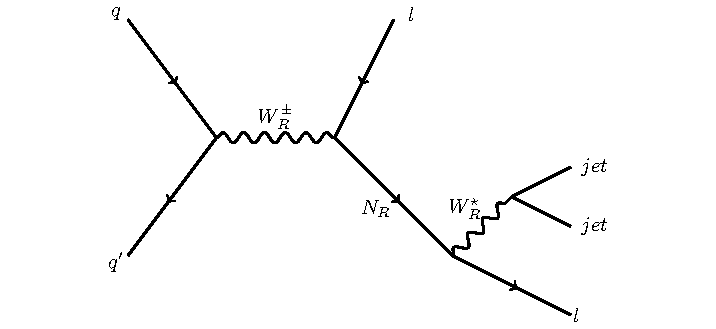
\includegraphics[width=1.0\textwidth]{figures/feynman.pdf}
	\caption{Production of a \WR boson and its decay to two charged leptons and two quarks through 
	a heavy neutrino \nul.}
	\label{fig:wrFeynmanDiagram}
\end{figure}

%%%%%%%%%%%%%%%%%%%%%%%%%%%%%%%%%%%%%%%%%%%%%%%%%%%%%%%%%%%%%%%%%%%%%%%%%%%%%%%%
